\section{Potential Solutions}
\label{solutions}
This section outlines several potential solutions for how to let Ursula prove 
that she served a given number of distinct requests in a publicly verifiable way. 
One of these solutions, the PCD-based one, is still a work in progress. The goal 
is to share the high-level idea of each of these solutions and to chose the best one,
after we define the meaning of best, to be adopted by the NuCypher network.


\subsection{PCD-based Scheme}
The main idea here is to adapt the PCD framework so that Ursula
can combine the correctness proofs she computes for Bobs' requests in a single proof 
attesting to the following fact: ``Ursula has served $\omega$ distinct re-encryption 
requests correctly." 


Thus, in this setup, there is only one computation party, or prover, namely, Ursula. 
For each round, where a round could be the time needed to mine a block on the 
blockchain, Ursula starts with input $x_1$, which is a signed and fresh request
from Bob. It answers this request with $cFrag_{x_1}$ and produces a correctness 
proof $\pi_1$ as defined in the Umbral scheme, in addition to another correctness 
proof $\hat{\pi}_1$ that will be used in the PCD composition. Then, when the next request $x_2$ arrives, 
which is the input for the next step in the computation, Ursula answers 
this request as before and produces $cFrag_{x_2}$ and a correctness proof $\pi_2$, then 
it uses $(x_2, cFrag_{x_2}, \pi_2)$ and the previous proof $\hat{\pi}_1$ to produce $\hat{\pi}_2$. 
$\hat{\pi}_2$ does not only 
attest to the correctness of $cFrag_{x_2}$, but also attests to the fact that Ursula has served 
two valid distinct requests until now. The same process is repeated until the end of the 
round to produce a single proof $\hat{\pi}_{\omega}$ along with the number of 
served requests $\omega$. Figure~\ref{pcd-based-sol} depicts 
this process pictorially.


\begin{figure}[h!]
\centerline{
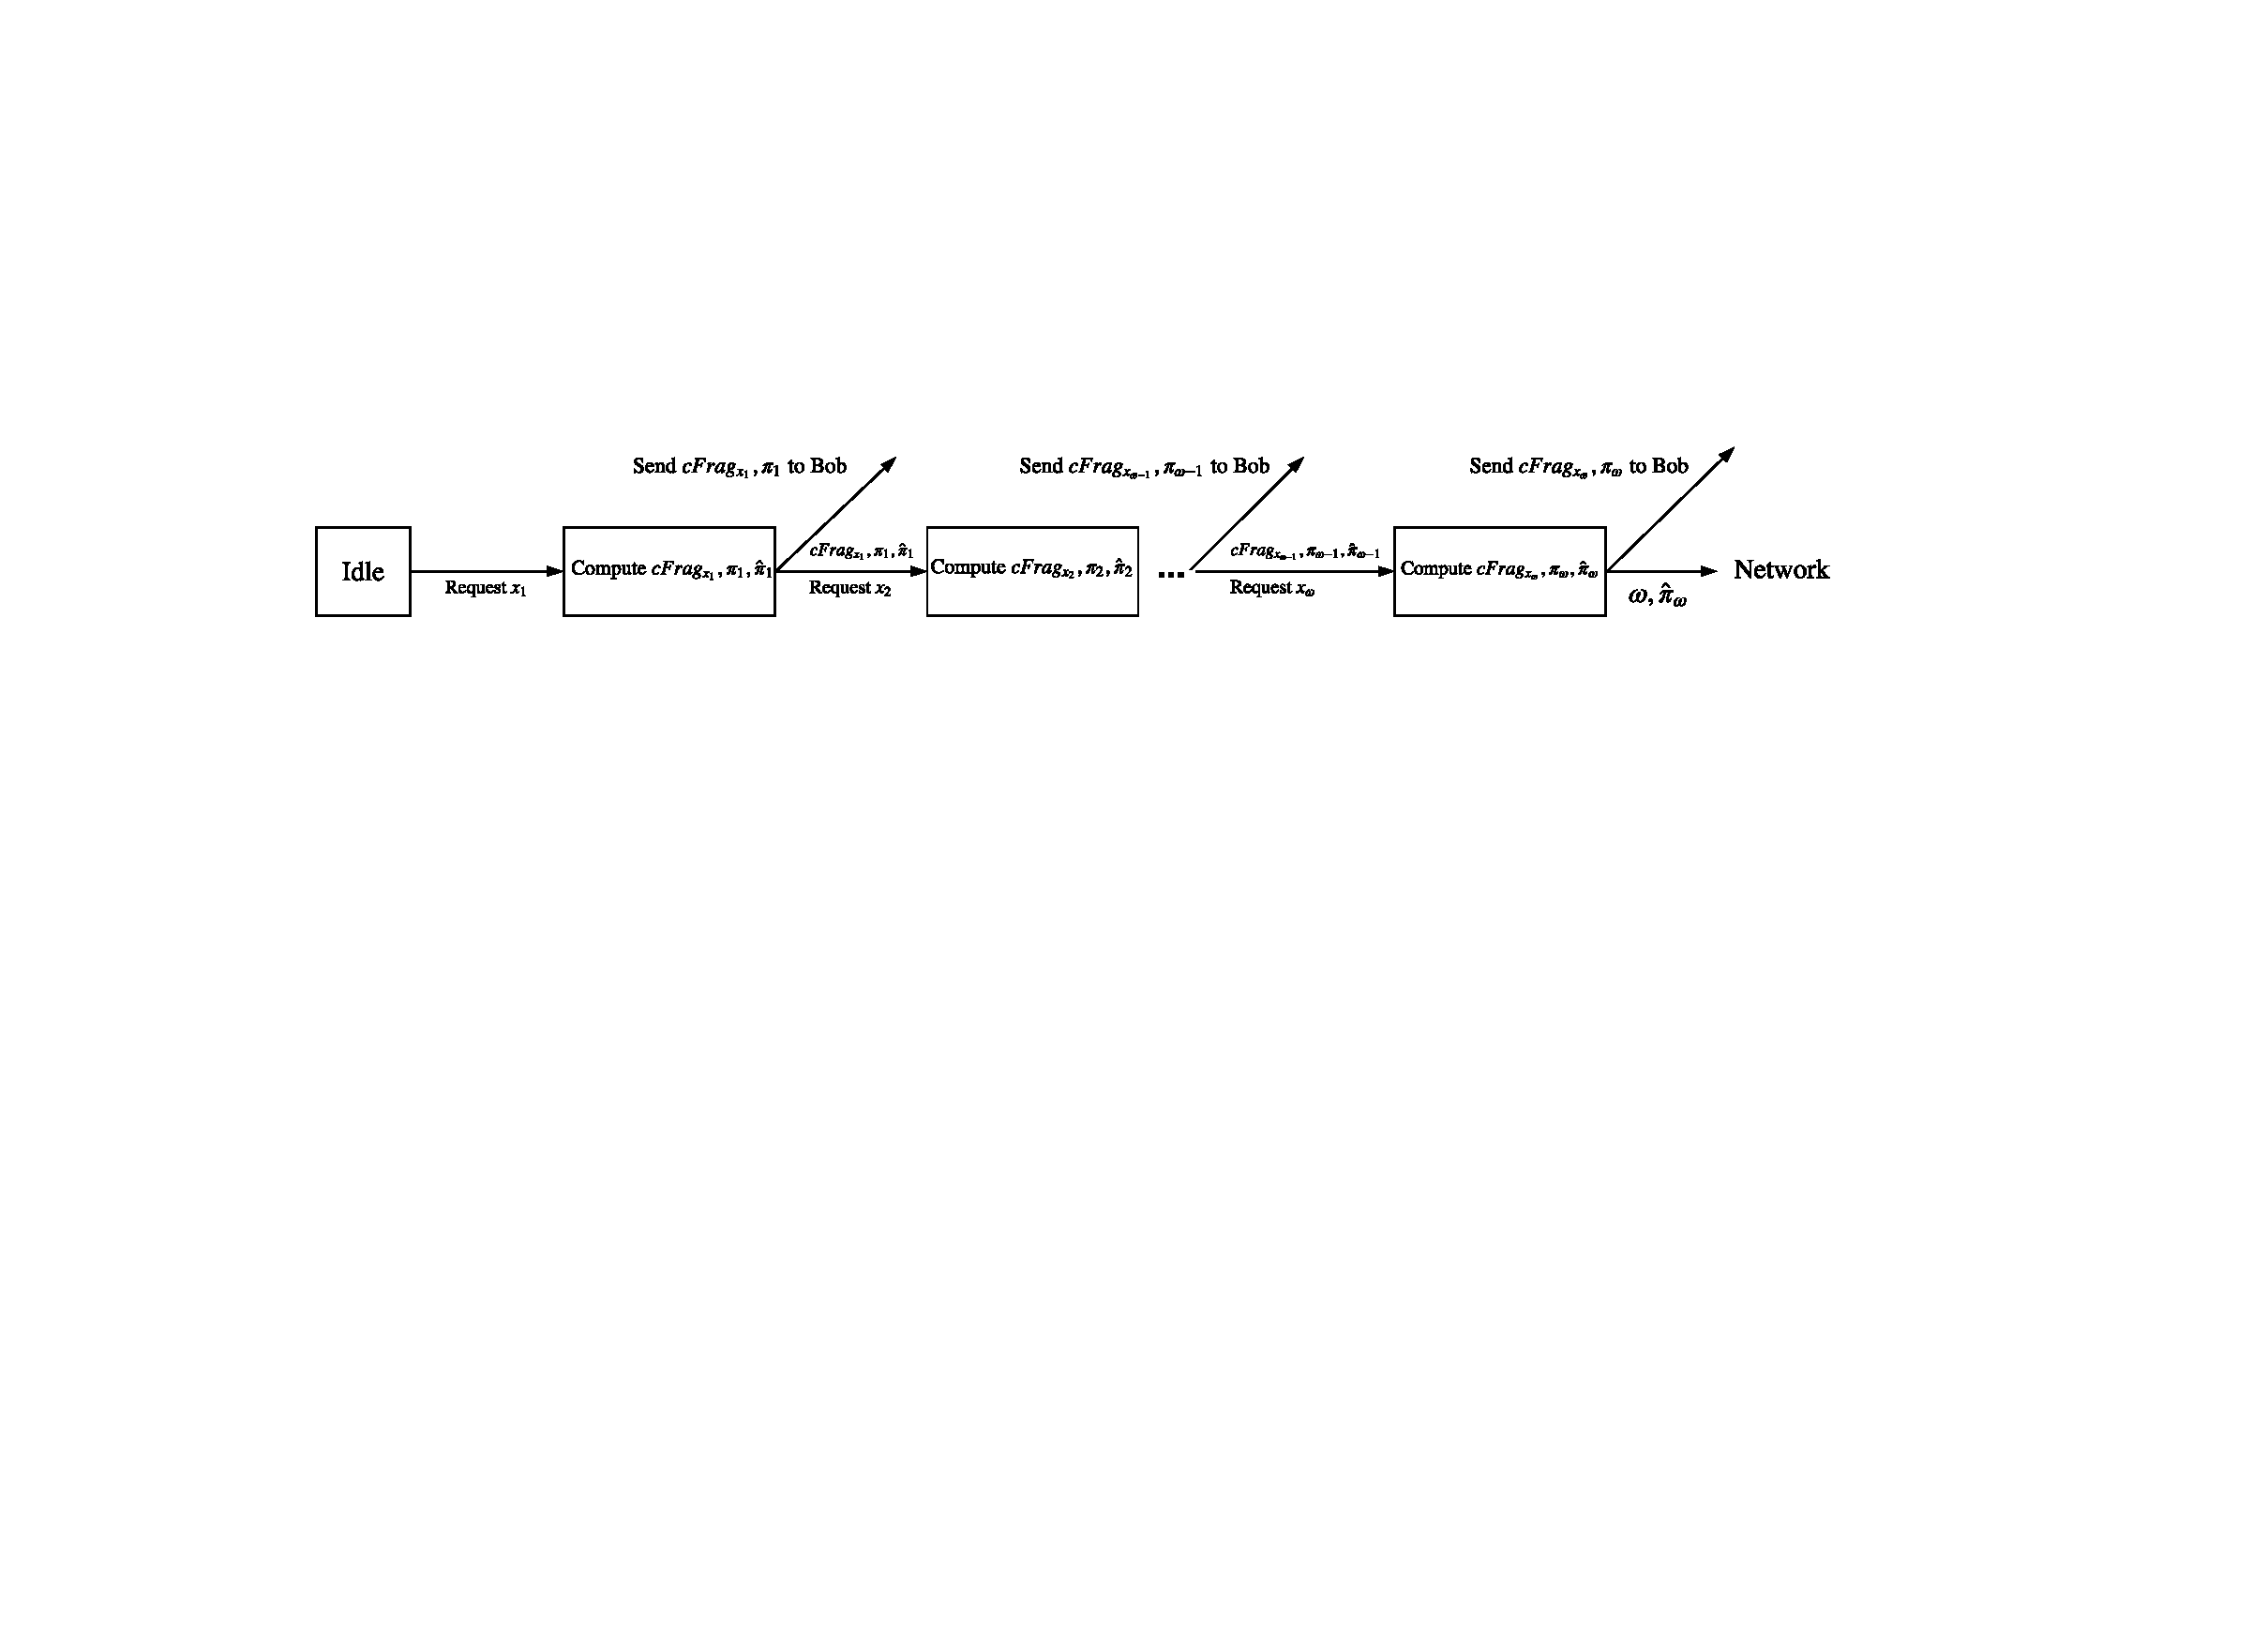
\includegraphics[height= 0.7in, width = 1.0\columnwidth]{figures/pcd-based-sol.pdf}}
\caption{PCD-based solution diagram. Ursula starts a round in the idle state. When 
the first request arrives, Ursula responds to the request and starts composing the 
proofs as new requests arrive. At the end of the round, Ursula announces the number of 
served requests and a single proof attesting to its claim to the network. }
\label{pcd-based-sol}
\end{figure}


The final proof will be processed by the contract that governs Alice's policy. A valid proof 
allows Ursula to claim fees out of Alice's Ether escrow as a payment for $\omega$ re-encryption  
requests. 


The above is a high level description of the idea. However, more time is need to 
understand PCD and SNARKs in order to come up with a concrete construction 
(if possible). Please see Section~\ref{future-work} for more information.

\david{I think it is possible to aggregate current Umbral proofs. I started to explore this option in the past but there was no use for it at that moment.}

\subsection{CoSi-based Scheme}
This solution utilizes the idea of collective signing by electing a committee 
that will sign a report submitted by a specific Ursula after verifying that 
the report supports the claim that ``Ursula has served $\omega$ distinct 
re-encryption requests correctly." 


At a high level, the scheme works as follows. For each round, a working Ursula keeps 
a full record of all the requests that she served during the round. These 
include the signed requests received from Bob(s), and the produced $cFrag$ 
and the correctness proof $\pi$ (as in the Umbral scheme) for 
each request. At the end of the round, a committee of $t$ Ursulas is 
elected, where $t$ is a small integer, e.g., $t = 5$. The working Ursula 
initiates the CoSi protocol to sign the message $m$ stated above while 
replacing $\omega$ with the actual number of served 
requests in the round. This Ursula sends $m$ along with the full report to 
each member in the committee. Each member Ursula (i.e., member in the 
elected committee) verifies $m$ by checking the report as follows:
\begin{enumerate}
\setlength{\itemsep}{0pt}
\item Check that each request is distinct and valid by verifying Bob's 
signature over the request. (Here the policy will contain Bob's public 
key to allow the committee use the right verification key.)

\derek{Signature only validates request, but for distinct requests, presumably blockhash/sequence number needs to also be checked?}

\item Verify the correctness of each $cFrag$ as in the Umbral 
scheme.

\item Check that the value of $\omega$ inside $m$ agrees with the 
record.
\end{enumerate}


If everything is fine, each member of the committee and the working 
Ursula finalize the CoSi signing protocol as described in Section~\ref{cosi}. 
At the end, the working Ursula publishes the collective signature, which can be 
verified using the accumulated public keys of the cosigning Ursulas.


\subsubsection{On the committee election.} This can be done
by using some deterministic computation over a block hash and mapping
the output to Ursulas' public keys. So the selection is not determined by the
working Ursula to prevent any potential collusion. The selection may also take into account the presence and size of each Ursula's stake, to avoid an attacker spinning up enormous numbers of Ursulas in order to increase the chance of them controlling the entire committee.


The above scheme works under the assumption that at least one Ursula
in the elected committee is honest, which pertains to an assumption on the
least number of honest Ursulas in the network. If the latter assumption is under threat, one mitigating approach is to increase $t$ (the committee size).


Another approach is to have a changing set of external verifiers, like
trusted partners, that all working Ursulas must use for the CoSi signing
of their records.


A third approach is to keep the deterministic selection of the committee
but with an external member, e.g., either a trusted partner verifier
or a special verifier node deployed and maintained by the NuCypher company.
Thus, achieving the assumption of at least one member of the elected
committee is honest.


\subsubsection{On the publicity of the signed records.} Having a 
valid collective signature from a committee (that has at least one honest 
member) suffices for the correctness of the signed statement. However, 
it could be better to keep the records that produced the message $m$  
available for a while so that any party can verify them (the verifying
parties could maintain such a public record for a given period after which
the logs can be discarded). 


We can resort to this option just at the beginning to convince the 
participants of the trustworthiness of the committee or the validity of the
assumption that at least one Ursula in the elected committee is honest.


\subsubsection{On compensating the committee.} This solution may 
raise the question of why would the elected committee (especially if it 
is composed of other Ursulas in the system) participate in the CoSi 
process, which also involves verifying the full request record presented 
by the working Ursula. This can be pictured as a collaborative
work, the committee does the work so that others will do the same
when the committee members play the role of working Ursulas.


Another option is to pay the committee for their work, either as
part of the inflation rewards, or by having working Ursulas pay for 
it (however, this may complicate the system operation).


\subsection{Challenge/Open-based Scheme}
This solution utilizes the idea of commit/challenge/open protocols. 
In details, Ursula keeps track of the requests coming from Bob(s) 
during a time round and assign each of them a unique sequence 
number. That is, Ursula replies with $cFrag$ and the correctness proof 
along with a sequence number showing the order of the request within 
the batch of requests handled during a round. At the end of the round, 
Ursula constructs a Merkle tree of all requests, where 
the requests (and their replies) are the leaves of the tree ordered by the sequence
numbers. Ursula signs the root of the tree, denoted as $root$ to produce 
a signature $\sigma_{root}$, then it publishes $(\omega, root, \sigma_{root})$ 
to the network (recall that $\omega$ is the number of served requests). 


To prove correctness, Ursula will be challenged to open some leaves in the Merkle tree. 
This can be done by having the policy contract select at random (e.g. based
on the block hash or any other mechanism) the leaf IDs to be opened. If 
Ursula fails to open them correctly within a predefined timeframe, she loses the 
whole fee she was supposed to collect for serving $\omega$ requests.


An alternative approach to the challenge/open scheme described above is to 
have Ursula publish the full Merkle tree on some known public space but
not on the blockchain, and make the full record available online for a specific period
to allow anyone to verify the work. If no one files a complaint about the tree (we
still need to define correctness properties, like checking all Bob public keys are 
defined in the policy created by Alice, and that the response is valid by checking the 
proof produced by Umbral), Ursula collects the fees for the provided service. On the other
hand, a valid complaint or proof-of-cheating costs Ursula the full allocation of fees, or potentially involves slashing her stake.